\chapter{Analysis}\label{ch:Analysis}
\label{ch:TrackingLoops}


In summary, the goal of the carrier tracking loop is to predict the future carrier phase $\phi$, $T$ seconds in the future, based on past and current measurements of the carrier phase. For successful phase lock to be maintained, the predicted phase must be within a small fraction of a cycle of the actual phase. 

\section{Ambiguities}

We can describe the elapsed phase (in radians) between the satellite and the receiver using the following equation :  
\begin{equation}
Phase = 2 \pi N  + \phi 
\label{eq:Phase}
\end{equation}

If we examine equation \ref{eq:Phase} in the spatial domain, we find that: 
\begin{equation}
Range = \lambda N + \Phi
\label{eq:Distance}
\end{equation}

From Equations \ref{eq:Phase} and \ref{eq:Distance} it is obvious that prediction of the angular phase $\phi$ is equivalent to prediction of the spatial phase $\Phi$.

It is important to note, that predicting $\Phi$ is equivalent to predicting the change in the LOS range ($\Delta$), hence the receiver does not need to be aware of the number of full cycles $N$, between it and the satellite. This ambiguity is the one that is resolved during the process of carrier phase positioning. 

\section{Error bounds}
In the case of the GPS signal, where the $L_1$ 1.575Ghz signal is being tracked, the carrier wavelength, $\lambda \approx 19.03 cm$ long. As a heuristic, the difference between the actual carrier phase $\phi$ , and the predicted carrier phase $\hat{\phi}$ must be no more than $\pm30 \degree$. 

This concept is clearly illustrated in figure \ref{fig:PhaseDelay}. 

Denoting our prediction of $\Delta$ as $\hat{\Delta}$, we have :

\begin{align}
|\Delta-\hat{\Delta}|& < \frac{30\degree}{360\degree} \lambda\\
|\Delta-\hat{\Delta}|&<\epsilon\\
|\Delta-\hat{\Delta}|&<1.58cm\\
\label{eq:RangeErrorBound}
\end{align}

Hence, our estimate of $\Delta$ must be accurate to $< 1.58cm$, if the receiver is to remain in phase lock.

By examining figure \ref{fig:ValidPositions} we can begin to understand that the locus of all possible positions which meet this criteria is a spherical shell surrounding the satellite. 

When we consider that GPS utilises multiple satellites for positioning, we can conclude with the aid of figure \ref{fig:Intersections} that a bound on the magnitude of the error is formed by the sphere of radius $\epsilon$ surrounding the point X, which is the true position of the receiver. 

\begin{comment}

Hence, we have :

\begin{align}
| X(t)-\hat{X}(t) | & < \frac{30\degree}{360\degree} \lambda \\
| X(t)-\hat{X}(t) | &<\Delta\\
| X(t)-\hat{X}(t) | & < 1.58cm
\label{eq:PositionErrorBound}
\end{align}
\end{comment}

\section{Mechanics}

By conceptualising we can immediately gain insight into some of the fundamental challenges that will be faced in the development of tracking algorithms for coping with high dynamics.

\tikzset{
block/.style = {draw, fill=white, rectangle, minimum height=3em, minimum width=3em},
tmp/.style  = {coordinate}, 
sum/.style= {draw, fill=white, circle, node distance=1cm},
input/.style = {coordinate},
output/.style= {coordinate},
pinstyle/.style = {pin edge={to-,thin,black}
}
}

\begin{figure}[!htb]
\centering

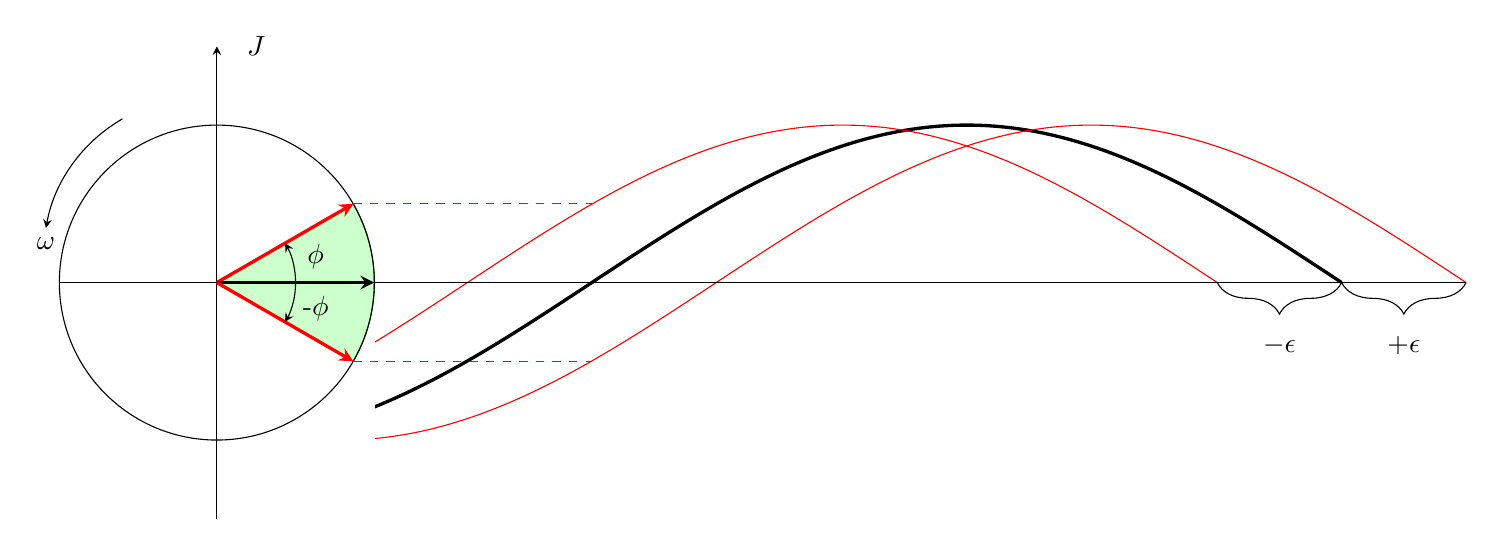
\begin{tikzpicture}
    
    \draw[black,very thick] (0,-2) cos (4.76175,0) sin (2*4.76175,2) cos (3*4.76175,0) ;
    
    \draw[red] (-1.58,-2) cos (4.76175-1.58,0) sin (2*4.76175-1.58,2) cos (3*4.76175-1.58,0) ;
    
    \draw[red] (1.58,-2) cos (4.76175+1.58,0) sin (2*4.76175+1.58,2) cos (3*4.76175+1.58,0) ;
    
    \draw [decorate,decoration={brace,amplitude=0.4cm},xshift=0,yshift=0pt]
(3*4.76175+1.58,0) -- (3*4.76175,0) node [black,midway]{};
    \node at (3*4.76175+0.5*1.58,-0.8) {$+\epsilon$};
    
    \draw [decorate,decoration={brace,amplitude=0.4cm,mirror},xshift=0,yshift=0pt]
(3*4.76175-1.58,0) -- (3*4.76175,0) node [black,midway]{};
    \node at (3*4.76175-0.5*1.58,-0.8) {$-\epsilon$};

    \draw [fill opacity=1, fill=white,white] (-1.58,0.1) rectangle(2,-2.1);
    
    \filldraw[fill=green!20!white, draw=green!50!black]
    (0,0) -- (-30:2) arc (-30:30:2) -- cycle;
    \draw (0,0) circle (2cm);
    
    \draw[->,-stealth,color=black] (0,-3) -- (0,3);
    \node at (0.5,3) {$J$};
    
    \draw(-2,0) -- (3*4.76175+1.58,0);
    
    \draw[->,color=red, very thick,-stealth] (0,0)--(30:2);
    \draw[->,color=black, very thick,-stealth ] (0,0)--(0:2);
    \draw[->,color=red, very thick,-stealth ] (0,0)--(-30:2);
    
    \draw[-,color=red, dashed] (30:2)--(4.76175,1);
    \draw[-,color=red, dashed] (-30:2)--(4.76175,-1);
    
    \draw[->,-stealth ]  (0:1cm) arc (0:30:1cm);
    \draw[->,-stealth ]  (0:1cm) arc (0:-30:1cm);
    
    \node at (15:1.3) {$\phi$};
    \node at (-15:1.3) {-$\phi$};
    % angular velocity \omega
    \draw[->,-stealth ]  (120:2.4cm) arc (120:170:2) node[below] {$\omega$};
    
    \end{tikzpicture}
\caption{A scale drawing of the tolerances required for successful phase lock of the GPS $L_1$ signal.The phase, $\phi$ of the locally generated carrier (red) needs to remain within $30\degree$ of the phase the incoming carrier (black). This equates to a $\Delta$ range of 1.58 cm to the satellite.} \label{fig:PhaseDelay}
\end{figure}


\tikzset{
block/.style = {draw, fill=white, rectangle, minimum height=3em, minimum width=3em},
tmp/.style  = {coordinate}, 
sum/.style= {draw, fill=white, circle, node distance=1cm},
input/.style = {coordinate},
output/.style= {coordinate},
pinstyle/.style = {pin edge={to-,thin,black}
}
}

\begin{figure}[!htb]
\centering

\begin{tikzpicture}
    \newcommand\Radius{6} 
    \filldraw[fill=green!20!white, draw=green!50!black]
    (0:\Radius+1.58) arc (0:360:\Radius+1.58) -- cycle;
    
    \filldraw[fill=white, draw=green!50!black]
    (0:\Radius-1.58) arc (0:360:\Radius-1.58) -- cycle;
    
    \draw[draw=green!50!black,dashed]
    (0:\Radius) arc (0:360:\Radius) -- cycle;
    
    \draw[->,color=black,-stealth, thick] (0,0)--(30:\Radius+1.58);
    \draw[->,color=black,-stealth, thick] (0,0)--(90:\Radius);
    \draw[->,color=black,-stealth, thick] (0,0)--(150:\Radius-1.58);
    
    
    \node at (20:3) {$r+\Delta$};
    \node at (95:3) {$r$};
    \node at (160:3) {$r-\Delta$};
    \node at (0,-0.25) {Satellite};
    
    \end{tikzpicture}
\caption{In order to maintain phase lock with a single satellite, the predicted range to the satellite used to generate the phase, must lie inside an spherical shell, centred around the true range to the satellite. The shell is visualised as an annulus which is bounded by $r-\epsilon<r<r+\epsilon$. $\epsilon$ is depicted at 1:1 scale.} \label{fig:ValidPositions}
\end{figure}


\tikzset{
block/.style = {draw, fill=white, rectangle, minimum height=3em, minimum width=3em},
tmp/.style  = {coordinate}, 
sum/.style= {draw, fill=white, circle, node distance=1cm},
input/.style = {coordinate},
output/.style= {coordinate},
pinstyle/.style = {pin edge={to-,thin,black}
}
}

\begin{figure}[!htb]
\centering

\begin{tikzpicture}
    %\filldraw[fill=green!20!white, draw=green!20!white]
    %(-59.5:7.58) arc (-59.5:-120.5:7.58) arc (147:32:4.58) %--cycle;
    
    \filldraw[fill=green!20!white, draw=green!20!white]
    (-46:5.58) arc (-46:-134:5.58) arc (134.5:46:5.58);
    
    
    \newcommand\RadiusA{4} 
    \draw[draw=black]
    (0:\RadiusA+1.58) arc (0:360:\RadiusA+1.58) -- cycle;
    
    \draw[draw=black]
    (0:\RadiusA-1.58) arc (0:360:\RadiusA-1.58) -- cycle;
    
    \draw[draw=black,dashed]
    (0:\RadiusA) arc (0:360:\RadiusA) -- cycle;
    
    \node at (0,0) {Satellite A};
    
    \newcommand\RadiusB{4} 
    \draw[draw=black]
    (\RadiusB+1.58,-8) arc (0:360:\RadiusB+1.58) -- cycle;
    
    \draw[draw=black]
    (\RadiusB-1.58,-8) arc (0:360:\RadiusB-1.58) -- cycle;
    
    \draw[dashed]
    (\RadiusB,-8) arc (0:360:\RadiusB) -- cycle;
    
    \node at (0,-8) {Satellite B};
    
    \node at (0,-4.35) {$X$};
    
    \end{tikzpicture}
\caption{In the case of multiple satellites, the only viable positions where phase lock can be maintained is the union between the spherical shells of the satellites, visualised here as annuli. As the number of different satellites increases, the bounding volume of the solution approaches a sphere with radius 2 $\epsilon$ centred at the true position X. $\epsilon$ is depicted at 1:1 scale.}
\label{fig:Intersections}
\end{figure}



Returning to first principles of mechanics, we have \cite{salas1999etgen} : 

\begin{comment}
Need to fix this up
\end{comment}

\begin{align}
v & = \frac{\Delta}{T} m s^{-1} \\
a & = \frac{dv}{dt} m s^{-2} \\
Jerk & = \frac{da}{dt} m s^{-3}
\end{align}


Note that over time, the acceleration of the receiver is integrated to form it's velocity, and the velocity is integrated in order to form it's position. 

Note that our estimate of the position $\hat{X}(t+T)$ is dependent on our current velocity $\dot{X}(t)$. When use this velocity, we are implicit assuming that the average velocity for the next time period is the same. 

However,as illustrated in figure \ref{fig:PhaseDelay}, and in equation \ref{eq:RangeErrorBound}, our estimate of the new range to the satellite must fall within 
position must fall within a close 

our estimate of the velocity must fall within the following bounds:

\begin{equation}
V_{min} < \hat{\dot{X}}(t) < V_{max}
\end{equation}

\section{Motion models}

Given we are attempting to predict the carrier $T$ seconds into the future, we can start to investigate the maximum dynamics our receiver will be able to track for a given sampling period $T$. \cite{salas1999etgen}


\begin{equation}
X = \int_{t_1}^{t_2} \dot{X} dt + X(t_1)
\label{eq:PositionIntergral}
\end{equation}

\begin{equation}
\dot{X} = \int_{t_1}^{t_2} \ddot{X} dt + \dot{X}(t_1)
\end{equation}


Equation \ref{eq:PositionIntergral} suggests that we can form an prediction of the range to the satellite using the current range and the current line of sight velocity. 

\begin{equation}
\hat{X}(t+T) = X(t) +  \dot{X}(t) T
\end{equation}

\begin{equation}
t = nT
\end{equation}

\begin{equation}
\hat{X}[n+1] = X[n] +  \dot{X}[n] T
\end{equation}




\section{Current \ac{NAMURU} architecture}
A significant amount of time has been invested gaining an understanding of the \ac{NAMURU} receiver, its architecture and the operation of it's sub-systems. The receiver is a mixed signal device, which has been the focus of a decade of research and development. 

A detailed understanding of the receiver is crucial, if it is to be accurately modelled, in particular the ways that non idealities cause the performance of the receiver to deviate from analog models. For example, delays and jitter introduced  by the receiver's \ac{RTOS}. The Aquarius firmware developed by Glennon \cite{Glennon11aquariusfirmware} implements the tracking loop algorithm using 4,100 lines of optimised C, illustrating the complexity of the implementation.

The \ac{NAMURU} receiver uses a number of different tracking loops to track the incoming signal. During operation, the receiver transitions between a number of different states, choosing the most appropriate tracking loop at each point in time. A thorough overview of the different tracking loops employed by the receiver can be found in appendix \ref{ch:StateTransitions}. Particular attention has been paid in this thesis to the type 3 PLL/ type 2 FLL which represents the final state for the tracking system. The type 3 PLL uses a 2nd order filter, while the type 2 FLL uses a 1st order filter. This filter architecture can be observed in figure \ref{fig:TrackingLoopeOverview}. 

\input{Diagrams/MyWork/ReceiverOverviewAnalog}

After conducting a literature review, it was decided to model the control loops used by the \ac{NAMURU} receiver in the Laplace domain. The choice of the coefficients from the tracking loop comes from a method devised by Ward \cite{Ward}. While this method is conceptually simple, requiring only a loop order and noise bandwidth as parameters, it generates robust tracking loops for most applications. Because of this, the Ward method has experienced significant popularity amongst receiver designers.  

The method used by Ward for design will be described below for context: 


\subsection{\ac{PLL} filter}
Ward's method is also used to design the co-efficients for the \ac{PLL}. In the Laplace domain, we can represent the second order filter  of the third order \ac{PLL} as : 

\begin{equation} \label{eq6}
G(s) = K_1 + \frac{K_2}{s} + \frac{K_3}{s^2}
\end{equation}

A loop bandwidth of 18Hz was originally chosen for the \ac{PLL}, as Kaplan\cite{Kaplan} demonstrated, using a Monte Carlo simulation, that higher loops bandwidths typically result in unstable behaviour. However the limiting factor for stability is the loop noise bandwidth time product. Kaplan uses an integration time of 20ms, resulting in a $B_LT$ of 0.36. Conversely \ac{NAMURU} uses an integration time of 8ms, which means that any loop noise bandwidth $\leq 45$ can be used. 

Using Ward's method\cite{Ward} for finding $K_1,K_2 \& K_3$:

\begin{align*}
B_n &= 18\\
a_3&=1.1\\
b_3&=2.4\\
\omega_{0}&=\frac{B_n}{0.7845}
\end{align*}

\begin{align*} \label{eq3}
K_3 & = b_3 \omega_{0}\\
    & = 55.1\\
K_4 & = a_3 \omega_{0}^2\\ 
    & = 579.13\\
K_5 & = \omega_{0}^3\\
    & = 12079
\end{align*}


\subsection{\ac{FLL} filter}
In the Laplace domain, we can represent the second order \ac{FLL} filter as:  $G(s) = K_1 + \frac{K_2}{s}$. The design method from Ward \cite{Ward} is used in order to determine the coefficients $K_1$ and $K_2$.  

\begin{align*}
B_n &= 6\\
a_2 &= \sqrt(2)\\
\omega_{0}&=\frac{B_n}{0.53}\\
\end{align*}

\begin{align*}
K_1 & = a_2 \omega_{0}\\
    & = 16.00\\
K_2 & = \omega_{0}^2\\
    & = 128.16
\end{align*}

\clearpage

\section{Combining FLL \& PLL}

The structure described by Ward is a combination of FLL/PLL, which operate in conjunction. This structure, which is described by Ward in his seminal paper  may initially give the impression that the FLL and PLL act independently, however a critical analysis in the Laplace domain shows that they are intricately linked\cite{Ward}.

The philosophy behind Ward's design is that the FLL will bring the frequency estimate of the tracking loop to within locking range, at which point the PLL will bring the tracking loop into phase lock. Upon further scrutiny, it becomes apparent that the PLL \& FLL form a hybrid loop, which can be analysed in the Laplace domain.


Paying particular attention to figure \ref{fig:TrackingLoopeOverview}, we can observe the PLL and FLL arms of the loop controller. The blocks $D_{PLL}$ and $D_{FLL}$ represent the PLL and FLL discriminators respectively. More information about the implementation of these discriminators can be found in appendix \ref{ch:Discriminators}. 

\input{Diagrams/MyWork/ReceiverOverviewLaplace}

\tikzset{
block/.style = {draw, fill=white, rectangle, minimum height=3em, minimum width=3em},
tmp/.style  = {coordinate}, 
sum/.style= {draw, fill=white, circle, node distance=1cm},
input/.style = {coordinate},
output/.style= {coordinate},
pinstyle/.style = {pin edge={to-,thin,black}
}
}

\begin{figure}[!htb]
\centering
\begin{tikzpicture}[auto, node distance=2cm,>=latex']
    \node [input, name=rinput] (rinput) {};
    \node [sum, right of=rinput,node distance = 2
    cm](Rotator){\Large$+$};
    \node [input, right of = Rotator] (RotatorPickoffPoint) {};
     
    
    
    %FLL Stuff
   
    \node [block, right of=Rotator,node distance =4cm] (SamplingTime){$\frac{1}{T}$};
    
    \node [block, below of = SamplingTime,node distance =8cm](K1FLL){$K_{1}$};
    
    \node [block, below of = K1FLL](IntegratorFLL){$\frac{1}{S}$};
    \node [block, left of = IntegratorFLL](K2FLL){$K_{2}$};
    \node [sum, left of=K1FLL,node distance=2cm] (sum1FLL) {\Large$+$};
    \node [sum, left of = sum1FLL,node distance =2cm](sumCommon){\Large$+$};
    
    \node [block, above of = VCOIntegrator](VCOGain){$K_{VCO}$};
    \node [block, above of = VCOGain](VCO){$\frac{1}{S}$};
    
    
    \node [input, right of = K1FLL] (FLLPickoffPoint) {};
    
    
    
    %PLL Stuff
    \node [block, above of=SamplingTime] (DiscriminatorPLL) {$1$};
    
    \node [block, left of = diffPLL](K1PLL){$K_{3}$};
    \node [block, below of = diffPLL](K2PLL){$K_{4}$};
    \node [block, right of = K2PLL](ExtraIntegrator){$\frac{1}{S}$};
    
    \node [block, below of = K2PLL](IntegratorPLL){$\frac{1}{S^2}$};
    \node [block, left of = IntegratorPLL](K3PLL){$K_{5}$};
    \node [sum, left of=K2PLL,node distance=2cm] (sum1PLL) {\Large$+$};
    \node [output, right of=DiscriminatorPLL, node distance=4cm] (output) {};
     
    
    \node [input, right of = diffPLL,node distance =4cm] (PLLPickoffPoint1) {};
    \node [input, right of = K2PLL,node distance =4cm] (PLLPickoffPoint2) {};
    
    
    %Common
    \draw [->] (rinput) -- node{$\phi_{Input}$}(Rotator);
    
    %FLL Stuff
    \draw [-] (Rotator) -- node{$\phi_{Error}$} (RotatorPickoffPoint);
    \draw [->] (RotatorPickoffPoint) -- node{} (SamplingTime);
    
    
    \draw [-] (SamplingTime) -| node{} (FLLPickoffPoint);
    \draw [->] (FLLPickoffPoint) -- node{} (K1FLL);
    \draw [->] (FLLPickoffPoint) |- node{} (IntegratorFLL);
    \draw [->] (IntegratorFLL) -- node{} (K2FLL);
    
    \draw [->] (K1FLL) -- node{} (sum1FLL);
    \draw [->] (K2FLL) -- node{} (sum1FLL);
    \draw [->] (sum1FLL) -- node{} (sumCommon);
    
    
    %PLL Stuff
    \draw [->] (RotatorPickoffPoint) |- node{} (DiscriminatorPLL);
    
    \draw [-] (DiscriminatorPLL) -- node [name=y] {}(output);
    
    \draw [-] (output) -- node{} (PLLPickoffPoint1);
    \draw [-] (PLLPickoffPoint1) -- node{} (PLLPickoffPoint2);
    \draw [->] (PLLPickoffPoint1) -- node{} (K1PLL);
    \draw [->] (PLLPickoffPoint2) -- node{} (ExtraIntegrator);
    \draw [->] (ExtraIntegrator) -- node{} (K2PLL);
    
    \draw [->] (PLLPickoffPoint2) |- node{} (IntegratorPLL);
   

    \draw [->] (IntegratorPLL) -- node{} (K3PLL);
    %\draw [->] (diffPLL) -- node{} (K1PLL);
    
    \draw [->] (K1PLL) -- node{} (sum1PLL);
    \draw [->] (K2PLL) -- node{} (sum1PLL);
    \draw [->] (K3PLL) -- node{} (sum1PLL);
    
    
    \draw [->] (sum1PLL) -| node{} (sumCommon);
    \draw [->] (sumCommon) -- node{} (VCOGain);
    %\draw [->] (VCOIntegrator) -- node{} (VCOGain);
    \draw [->] (VCOGain) -- node{} (VCO);
    \draw [->] (VCO) -- node{$\phi_{VCO}$} node[pos=0.90] {$-$} (Rotator);
    
    

    \end{tikzpicture}
\caption{In this model, the integrator before the \ac{VCO} has been moved into the loop filter structure of the PLL. In the case of the FLL, the pole from the integrator has been cancelled with the zero from the differentiator in the FLL discriminator.} 
\label{fig:ModifiedStructure}
\end{figure}


\tikzset{
block/.style = {draw, fill=white, rectangle, minimum height=3em, minimum width=3em},
tmp/.style  = {coordinate}, 
sum/.style= {draw, fill=white, circle, node distance=1cm},
input/.style = {coordinate},
output/.style= {coordinate},
pinstyle/.style = {pin edge={to-,thin,black}
}
}

\begin{figure}[!htb]
\centering
\begin{tikzpicture}[auto, node distance=2cm,>=latex']
    \node [input, name=rinput] (rinput) {};
    \node [sum, right of=rinput,node distance = 2cm](Rotator){\Large$+$};
    \node [block, below of =Rotator](VCO){$\frac{1}{S}$};
    
    %PLL Stuff
  
    
    \node at (4,-6) [sum] (sum1PLL) {\Large$+$};
  
    \node [block, above of = sum1PLL](K1PLL){$\frac{K_{1}}{T} + K_{3}$};
    \node [block, right of = sum1PLL](K2PLL){$\frac{K_{2}}{T} + K_{4}$};
    \node [block, right of = K2PLL](ExtraIntegrator){$\frac{1}{S}$};
    
    \node [block, below of = K2PLL](IntegratorPLL){$\frac{1}{S^2}$};
    \node [block, left of = IntegratorPLL](K3PLL){$K_{5}$};
    
     
    
    \node [input, right of = K1PLL,node distance =6cm] (PLLPickoffPoint1) {};
    \node [input, right of = K2PLL,node distance =4cm] (PLLPickoffPoint2) {};
    
    
    %Common
    \draw [->] (rinput) -- node{$\phi_{Input}$}(Rotator);
    \draw [-] (Rotator) -| node{} (PLLPickoffPoint1);
    
    
    \draw [-] (PLLPickoffPoint1) -- node{} (PLLPickoffPoint2);
    \draw [->] (PLLPickoffPoint1) -- node{} (K1PLL);
    \draw [->] (PLLPickoffPoint2) -- node{} (ExtraIntegrator);
    \draw [->] (ExtraIntegrator) -- node{} (K2PLL);
    
    \draw [->] (PLLPickoffPoint2) |- node{} (IntegratorPLL);

    \draw [->] (IntegratorPLL) -- node{} (K3PLL);
   
    
    \draw [->] (K1PLL) -- node{} (sum1PLL);
    \draw [->] (K2PLL) -- node{} (sum1PLL);
    \draw [->] (K3PLL) -- node{} (sum1PLL);

    \draw [->] (sum1PLL) -| node{} (VCO);
    \draw [->] (VCO) -- node{$\phi_{VCO}$} node[pos=0.90] {$-$} (Rotator);
    
    \end{tikzpicture}
\caption{The reduced block diagram, to simplify the diagram, we assume that $K_{VCO}=1$.} 
\label{fig:ModifiedStructure2}
\end{figure}


From figure \ref{fig:ModifiedStructure2} we can find the open loop transfer function as:

\begin{equation}
G(s) = \frac{1}{s} (K_1+K_3 + \frac{1}{s}(K_2+K_4) + \frac{1}{s^2} K_5)
\label{eq:CombinedOpenLoopTF}
\end{equation}

We can convert the open loop transfer function $G(s)$ to the closed loop transfer function $H(s)$ as follows\cite{KazemiPHD,Gardner}:

\begin{equation}
 H(s) = \frac{K_{VCO}G(s)}{1+K_{VCO}G(s)}
\end{equation}

Assuming $K_{VCO}=1$:

\begin{equation}
 H(s) = \frac{G(s)}{1+G(s)}
\label{eq:OpenLoopToClosedLoop}
\end{equation}

Substituting equation \ref{eq:CombinedOpenLoopTF} into equation \ref{eq:OpenLoopToClosedLoop}:

\begin{equation}
 H(s) = \frac{\frac{1}{s} (K_1+K_3 + \frac{1}{s}(K_2+K_4) + \frac{1}{s^2} K_5)}{1+\frac{1}{s} (K_1+K_3 + \frac{1}{s}(K_2+K_4) + \frac{1}{s^2} K_5)}
\end{equation}

\begin{equation}
 H(s) = \frac{s^2(K_1+K_3) + s(K_2+K_4) + K_5}
 {s^3+ s^2(K_1+K_3)+ s(K_2+K_4) + K_5}
\end{equation}
\clearpage


From Wards method \cite{Ward}, we have the following coefficients:

\begin{align*}
K_1 &=\frac{\sqrt{2}B_{nFLL}}{0.53}\\
    &= 2.668 B_{nFLL}\\
K_2 &=\frac{B_{nFLL}^2}{0.53^2}\\
    &= 0.2809 B_{nFLL}^2\\
K_3 &=\frac{2.4B_{nPLL}}{0.7845}\\ 
    &=3.059 B_{nPLL}\\
K_4 &=\frac{1.1B_{nPLL}^2}{0.7845^2}\\
    &=1.787 B_{nPLL}^2\\
K_5 &=\frac{B_{nPLL}^3}{0.7845^3}\\
    &=0.4828B_{nPLL}^3
\end{align*}

It is clear at this point that the behaviour of the combined loop is entirely parametrised by $B_{nFLL}$,  $B_{nPLL}$ and $T$. $T$ is equal to the time between phase samples, which is currently 4ms for the \ac{NAMURU} receiver.

\subsection{Backward difference}

\begin{equation}
s \approx \Big(\frac{z-1}{Tz}\Big)
\end{equation}

\begin{comment}
\begin{equation}
 H(s) = \frac{s^2(K1) + s(K2) + K3}
 {s^3+ s^2(K1)+ s(K2) + K3}
\end{equation}

\begin{equation}
 H(s) = \frac{\Big(\frac{z-1}{Tz}\Big)^2(K1) + \Big(\frac{z-1}{Tz}\Big)(K2) + K3}{\Big(\frac{z-1}{Tz}\Big)^3+ \Big(\frac{z-1}{Tz}\Big)^2(K1)+ \Big(\frac{z-1}{Tz}\Big)(K2) + K3}
\end{equation}
\end{comment}

\begin{equation}
\frac{\frac{K_{1}}{t} + K_{3} + \frac{K_{5}}{s^{2}} + \frac{1}{s} \left(\frac{K_{2}}{t} + K_{4}\right)}{s \left(1 + \frac{1}{s} \left(\frac{K_{1}}{t} + K_{3} + \frac{K_{5}}{s^{2}} + \frac{1}{s} \left(\frac{K_{2}}{t} + K_{4}\right)\right)\right)}
\end{equation}

\begin{equation}
\frac{K_{1} s^{2} + K_{3} s^{2} t + K_{5} t + s \left(K_{2} + K_{4} t\right)}{K_{1} s^{2} + K_{3} s^{2} t + K_{5} t + s^{3} t + s \left(K_{2} + K_{4} t\right)}
\end{equation}

\begin{equation}
\frac{T z \left(K_{1} \left(z - 1\right)^{2} + K_{3} t \left(z - 1\right)^{2} + K_{5} T^{2} t z^{2} + T z \left(K_{2} + K_{4} t\right) \left(z - 1\right)\right)}{T z \left(K_{1} \left(z - 1\right)^{2} + K_{3} t \left(z - 1\right)^{2} + K_{5} T^{2} t z^{2} + T z \left(K_{2} + K_{4} t\right) \left(z - 1\right)\right) + t \left(z - 1\right)^{3}}
\end{equation}

For 10,32 8ms CohInt and 8ms update rate

\begin{equation}
\frac{1.0 z \left(30.5 z^{2} - 57.9 z + 27.5\right)}{31.5 z^{3} - 60.9 z^{2} + 30.5 z - 1.0}
\end{equation}


\cite{arashBook}
\clearpage


\subsection{Bilinear}

\subsubsection{Transform}
\begin{equation}
\frac{2 z - 2}{T \left(z + 1\right)}
\end{equation}

OL TF BN = 32,10

\subsubsection{S Domain open loop}
\begin{equation}
\frac{1}{s} \left(\frac{K_{1}}{t} + K_{3} + \frac{K_{5}}{s^{2}} + \frac{1}{s} \left(\frac{K_{2}}{t} + K_{4}\right)\right)
\end{equation}

\subsubsection{Z Domain open loop}

\begin{equation}
\frac{T\left(z + 1\right) }{8 t \left(z - 1\right)^{3}} \left(4(K_{1}  + K_{3} t)  \left(z - 1\right)^{2}  + 2 T \left(K_{2} + K_{4} t\right) \left(z - 1\right) \left(z + 1\right) + K_{5} T^{2} t \left(z + 1\right)^{2} \right)
\end{equation}

\subsubsection{Z Domain open loop 2}
\begin{equation}
\frac{\left(z + 1\right)}{8 \left(z - 1\right)^{3}} \left(4(K_{1}  + K_{3} t)  \left(z - 1\right)^{2} + 2 t \left(K_{2} + K_{4} t\right) \left(z - 1\right) \left(z + 1\right) + K_{5} t^{3} \left(z + 1\right)^{2}\right)
\end{equation}


\subsubsection{S Domain Open Loop with values (32,10,8ms)}
\begin{equation}
\frac{1}{s^{3}} \left(3.43 \cdot 10^{3} s^{2} + 4.63 \cdot 10^{4} s + 6.79 \cdot 10^{4}\right)
\end{equation}


\subsubsection{Z Domain Open Loop with values (32,10,8ms,125Hz)}
\begin{equation}
\frac{14.5 z^{3} - 13.0 z^{2} - 14.5 z + 13.0}{1.0 z^{3} - 3.0 z^{2} + 3.0 z - 1.0}
\end{equation}





\subsubsection{Z Domain closed loop}
\begin{equation}
\frac{T \left(z + 1\right) \left(4 K_{1} \left(z - 1\right)^{2} + 4 K_{3} t \left(z - 1\right)^{2} + K_{5} T^{2} t \left(z + 1\right)^{2} + 2 T \left(K_{2} + K_{4} t\right) \left(z - 1\right) \left(z + 1\right)\right)}{T \left(z + 1\right) \left(4 K_{1} \left(z - 1\right)^{2} + 4 K_{3} t \left(z - 1\right)^{2} + K_{5} T^{2} t \left(z + 1\right)^{2} + 2 T \left(K_{2} + K_{4} t\right) \left(z - 1\right) \left(z + 1\right)\right) + 8 t \left(z - 1\right)^{3}}
\end{equation}




For 10,32 8ms CohInt and 8ms update rate



\begin{equation}
\frac{14.5 z^{3} - 13.0 z^{2} - 14.5 z + 13.0}{15.5 z^{3} - 16.0 z^{2} - 11.5 z + 12.0}\end{equation}
\clearpage

\section{Forward difference}

\begin{equation}
\frac{K_{1} \left(z - 1\right)^{2} + K_{3} t \left(z - 1\right)^{2} + K_{5} t^{3} + t \left(K_{2} + K_{4} t\right) \left(z - 1\right)}{K_{1} \left(z - 1\right)^{2} + K_{3} t \left(z - 1\right)^{2} + K_{5} t^{3} + t \left(K_{2} + K_{4} t\right) \left(z - 1\right) + \left(z - 1\right)^{3}}
\end{equation}


For 10,32 8ms CohInt and 8ms update rate

\begin{equation}
\frac{6.71 \cdot 10^{9} z^{2} - 1.27 \cdot 10^{10} z + 5.99 \cdot 10^{9}}{2.44 \cdot 10^{8} z^{3} + 5.97 \cdot 10^{9} z^{2} - 1.2 \cdot 10^{10} z + 5.75 \cdot 10^{9}}
\end{equation}


\clearpage

\section{Ward analysis}

Ward introduces a number of incredibly useful rules of thumb for designing tracking loops for PLLs. 

From Kazemi, \cite{Kazemi2008}, the Loop Noise Bandwidth time product ($B_L T$) must be less than 0.55. 
For an 8ms integration time, corresponding to a 125Hz update rate we have:

\begin{align*}
B_n &\leq \frac{0.55}{0.008} \text{ (Hz)}\\
    &\leq 68.75 \text{ (Hz)}
\end{align*}

\subsection{PLL}
Kaplan suggests that "A conservative rule of thumb for tracking threshold is that the 3-sigma jitter must not exceed one-fourth of the phase pull-in range of the PLL discriminator"\cite{Kaplan}. This forms the basis of the "15 $\degree$" heuristic which is commonly used for analysis. Based on extensive experimental experience with the \ac{NAMURU} receiver, this heuristic has proved to be valuable in providing a rough estimate for the breaking point of the PLL. The 15 $\degree$ can be thought of an an error budget, which is eroded by different sources of error.

\begin{align}
3 \sigma_{PLL} &= 3 \sigma_j +\theta_e \leq 45 \degree\\
\sigma_{PLL} &=\sigma_j + \frac{\theta_e}{3} \leq 15 \degree
\end{align}

Where:
\begin{align*}
\sigma_j &= \text{1-sigma phase jitter from all sources except dynamic stress error} \\
\theta_e &= \text{dynamic stress error in the PLL tracking loop}
\end{align*}

Jwo breaks the equation down into more detail\cite{Jwo}, identifying the contributions to the error from the thermal noise in the signal as well as two contributions from the crystal, the vibration induced jitter and Allan variance intrinsic to the crystal.


\begin{equation}
\sigma_{PLL} = \sqrt{\sigma^2_{tPLL} + \sigma^2_v+ \theta^2_A} + \frac{\theta_e}{3} \leq 15 \degree 
\end{equation}

Where:
\begin{align*}
\sigma_{tPLL} &= \text{1-sigma thermal noise (degrees)}\\
\sigma_v &= \text{1-sigma vibration-induced oscillator jitter (degrees)}\\
\theta_A &= \text{Allan variance induced oscillator jitter (degrees)}
\end{align*}
%\cite{Kaplan}\cite{Jwo}


\begin{equation}
\sigma_{PLLt} = \frac{360}{2 \pi} \sqrt{\frac{B_n}{C/N_0}(1+\frac{1}{2 \cdot T \cdot C/N_0})} \text{ (degrees)}
\end{equation}
%\cite{Kaplan}

Where:
\begin{align*}
B_n &= \text{carrier loop noise bandwidth (Hz)} \\
C/N_0 &= \text{carrier to noise power ratio in (Hz)} \\
&=10^\frac{(C/N_0)_dB}{10} \text{ Hz}\\
T &= \text{pre-detection (coherent) integration time (s)} \\
\lambda_L &= \text{GPS L1 carrier wavelength (m)}\\
&= 0.1903 \text{ m}
\end{align*}



The dynamic stress error is due to the motion of the receiver, for a 3rd order PLL, the error is due to the \ac{LOS} jerk. The \ac{LOS} jerk is the projection of jerk vector onto the vector between the \ac{GPS} satellite and the receiver.  

\begin{equation}
\theta_e = \frac{360 \cdot Jerk  \cdot f_L}{c  \cdot \omega^3_0} \text{ (degrees)}
\end{equation}


Where:
\begin{align*}
\omega &= \frac{B_n}{0.7845} \\
f_L &= \text{L-band input frequency in Hz (1575.42MHz)}\\ 
c & = 2.99792458 \times 10^8 ms^{-1}
\end{align*}


Finally, the Allan variance is an error which is intrinsic to the crystal itself. 

\begin{equation}
\label{eq:AllanVariance}
\theta_{A3} = 160 \frac{\sigma_A(\tau)f_L}{B_n} \text{ (degrees)}
\end{equation}

From the data sheet for the current crystal used in the \ac{NAMURU} receiver\cite{VT803Datasheet}, we find that: 
\begin{align*}
\sigma_A(\tau) &= 1 \times 10^{-10} \text{ (dimensionless units of }\Delta f/f\text{)}
\end{align*}

Hence we can simplify equation \label{eq:AllanVariance} as:
\begin{equation}
\theta_{A3} =\frac{25.2}{B_n} \text{ (degrees)}
\end{equation}

For $B_n$ =18, we have $\theta_{A3}=1.4\degree$.


\begin{figure}[!htb] 
    \centering
    \includegraphics[width=1\textwidth]{mywork/18ContourPLL.eps} 
    \caption{A contour plot for a 3rd order loop with a $B_n$ of 18Hz. A value of $1.4\degree$ for the Allan variance oscillator jitter and $1.8\degree$ for vibration oscillator jitter is used. The conservative threshold of 15\degree can be seen in red. From this, we can conclude that the loop is likely to loose phase lock at a jerk of $150ms^{-3}$ given a $C/N_0$ of 30.}
\end{figure}

\begin{figure}[!htb] 
    \centering
    \includegraphics[width=1\textwidth]{mywork/32ContourPLL.eps} 
    \caption{A value of $1.4\degree$ for the Allan variance oscillator jitter and $1.8\degree$ for vibration oscillator jitter is used.}
\end{figure}


\begin{figure}[!htb] 
    \centering
    \includegraphics[width=1\textwidth]{mywork/PLLStresses.eps} 
    \caption{This plot breaks down the sources of error. Note that the phase jitter is at a minimum for a value of $B_n$ equal to approximately 27.}
\end{figure}


\section{Adaptive control}

No single controller can
optimally operate the PLL
under different conditions.
An algorithm was designed
which minimises the phase
jitter, by adapting the
coefficients of the tracking
loop controller and update
rates and integration times,
based on the cur rent
dynamics, SNR and the
vibration.
By adaptively adjusting the update rates, computation resources
are allocated to the tracking loops which are experiencing the
highest dynamics, and demand the highest controller
bandwidths.


In order to analytically determine the correct value of $B_n$, we can use the rules of thumb introduced by ward as a starting point. 





Optimising to find the minimum:

\begin{align*}
\sigma_{PLL} &= \sqrt{\frac{Bn}{C/N_0} \left(3280 + \frac{1640}{C/N_0 \cdot T}\right) + 4 + \frac{635}{Bn^{2}}} + \frac{304 Jerk}{Bn^{3}}\\
\sigma_{PLL}^2 &= \frac{Bn}{C/N_0} \left(3280 + \frac{1640}{C/N_0 \cdot T}\right) + 4 + \frac{635}{Bn^{2}} + \frac{Jerk^{2}}{Bn^{6}} 9.26 \cdot 10^{4}
\end{align*}


\begin{align*}
0&=\frac{1}{C/N_0} \left(3280 + \frac{1640}{C/N_0 \dot T}\right) - \frac{1}{Bn^{3}} 1.27 \cdot 10^{3} - \frac{Jerk^{2}}{Bn^{7}} 5.56 \cdot 10^{5}\\
0&=Bn^{7} \left(\frac{1}{C/N_0} \left(3280 + \frac{1640}{C/N_0 \cdot T}\right) - \frac{1}{Bn^{3}} 1.27 \cdot 10^{3} - \frac{Jerk^{2}}{Bn^{7}} 5.56 \cdot 10^{5}\right)\\
0&=\frac{3280 Bn^{7}}{C/N_0} + \frac{1640 Bn^{7}}{C/N_0^{2} \cdot T} - 1.27 \cdot 10^{3} Bn^{4} - 5.56 \cdot 10^{5} Jerk^{2}\\
0&=(\frac{3280}{C/N_0} + \frac{1640}{C/N_0^{2} \cdot T})Bn^{7}  - 1.27 \cdot 10^{3} Bn^{4} - 5.56 \cdot 10^{5} Jerk^{2}
\end{align*}

\subsection{FLL}


\begin{comment}
Talk about this
5.6.2 FLL Tracking Loop Measurement Errors

Generate figure 5.24
Generate figure 5.25

Also talk about section 5.6.2
\end{comment}

\begin{equation}\label{eq:FLLJitter}
\sigma_{FLL} =  \sigma_{tFLL} + \frac{f_e}{3} \leq \frac{T}{12} \text{ (Hz)}
\end{equation}

For T = 4ms, we have $\sigma_{FLL} \leq 20.83$ Hz.

Where:
\begin{align*}
\sigma_{tFLL} &= \text{1-sigma thermal noise frequency jitter}\\
f_e &= \text{dynamic stress error in the FLL tracking loop}
\end{align*}


\begin{equation}
\sigma_{tFLL} = \frac{1}{2 \pi T} \sqrt{ \frac{4FB_n}{C/N_0}(1 + \frac{1}{TC/N_0})} \text{ (Hz)}
\end{equation}

\begin{align*}
F &= \text{1 at high } C/N_0\\
  &= \text{2 near threshold}
\end{align*}


\begin{equation}
f_e = \frac{d}{dt}(\frac{1}{360 \omega^n_0}\frac{d^nR}{dt^n}) = \frac{1}{360\omega^n_0} \frac{d^{n+1}R}{dt^{n+1}} \text{ (Hz)}
\end{equation}


\begin{figure}[!htb] 
    \centering
    \includegraphics[width=1\textwidth]{mywork/1ContourFLL.eps} 
    \caption{A contour plot of equation \ref{eq:FLLJitter}. Note that the cutoff for the FLL is 20.83 Hz. }
\label{fig:FLLContour1}
\end{figure}

\begin{figure}[!htb] 
    \centering
    \includegraphics[width=1\textwidth]{mywork/10ContourFLL.eps} 
    \caption{A contour plot of equation \ref{eq:FLLJitter}. Comparing to figure \ref{fig:FLLContour1}, the significantly increased bandwidth allows the FLL to track significantly higher dynamics, for a given FLL jitter.}
\end{figure}



\begin{figure}[!htb] 
    \centering
    \includegraphics[width=1\textwidth]{mywork/FLLStresses.eps} 
    \caption{This plot breaks down the sources of error. Note that the phase jitter is at a minimum for a value of $B_n$ equal to approximately 27. Ideally the FLL bandwidth should be selected so that the FLL can always operate at this optimum point.}
\end{figure}



Significant preliminary work has been carried out, because of the challenging scope of thesis. 

In order to have a rigorous understanding of the dynamic performance of the \ac{NAMURU} receiver, we must first examine the theoretical basis for the operation of its tracking loops. 

A model of the operation of the tracking loops can be established by building upon intellectual foundations laid in continuous time control theory. While this Laplace domain model provides an idealised understanding of the \ac{PLL}, it does not take into the effects of delay and jitter in the loop. 

\ac{PLL}, \ac{FLL} and \ac{DLL} are all examples of control systems. By convention, what is referred to in the parlance of control theory as a "controller" is referred to as the "loop filter" in \ac{GNSS} related literature. One key point to keep in mind with a \ac{PLL} is that a phase input results in a frequency output. This effective integration occurs in the \ac{VCO}.

\section{Zeros and poles}
The behaviour of a closed loop system is determined by the locations of the zeros and the poles. An important caveat is that the location of the zeros and poles is for an analog model of the system, the locations will be different for a digital model, with the difference in location depending on the $B_LT$ product.  Hence it is possible to design a system which is stable in the Laplace domain but unstable in the Z Domain. 

Root locus provides an efficient graphical method for analysing the stability of a system in the Laplace domain\cite{Nise}. 


\begin{comment}
\begin{lstlisting}[frame=single]
Kvco =1;
Bn = 18;
a3 = 1.1;
b3 = 2.4;
omega = Bn/0.7845;
k1 = b3*omega;
k2 = a3*(omega^2);
k3 = omega^3;
%H is the forward transfer function
H = tf([Kvco*k1 Kvco*k2 Kvco*k3],[1 0 0 0]);
rlocus(H);
\end{lstlisting}
\end{comment}





